\documentclass[10pt,a4paper]{article}
\usepackage[margin=1.4cm]{geometry}
\usepackage[latin1]{inputenc}
\usepackage{amsmath}
\usepackage{amsfonts}
\usepackage{amssymb}
\usepackage{multirow}
\usepackage{graphicx}
\usepackage{subcaption}
\usepackage{morefloats}

\setlength{\parskip}{5pt}
\setlength{\parindent}{0pt}

\author{Hector Dearman \and Paul Rowe-White \and Kritaphat Songsriin \and Simon Stuckemann}
\title{Machine Learning CBC: Case-Based Reasoning\\Group 2}
\begin{document}
\maketitle

\section{Case-based Reasoning}
Contrary to the previous algorithms we have implemented (decision tree learning and artificial neural networks) which belong to the class of \emph{eager learning algorithms}, instance-based learning algorithms belong to the class  of so-called \emph{lazy learning methods}.
While \emph{eager learning algorithms} construct a general and explicit description of the target function when training examples are provided, \emph{lazy learning algorithms}, such as \emph{Case-based reasoning} simply store the training examples. Generalising beyond these examples is only done when a new instance must be classified. When a new instance should be classified, the algorithm compares the instance to the existing instances and assigns a target function value (the classification) based on the instance's relation to the already stored values. After classification of the new example, the \emph{CBR} system stores ("retains") the new example in order to use it for future classification. For this reason, the \emph{case-based} reasoning algorithm is also known as an \emph{online}-learning method as the algorithm continues to learn throughout its lifetime.

Throughout the report `RT' refers to Rogers and Tanimoto; `RR' to Russell and Rao; `SS' to Sokal and Sneath.

\section{Implementation Details}
In order to make it simpler to test and try new measures and CBR implementations
we used a pluggable system for implementing `retain' and the other operations.
Each operation calls an associated method handle on the CBR this allows us to change our whole implementation of CBR
and only have to change a single line in {\tt CBRinit.m}.
Similarly our CBR implementations take and a measure as an argument allowing us to easily change measures for testing.
What follows is an account of the implementation of our best CBR system, Nearest-k CBR.

\subsection{Case}
Our Case representation is a struct with three fields, the AUs in a list format,
the AUs in the bit vector\footnote{This was an optimisation to make calculating the similarity function faster.} and the solution (possibly null).
We do not count typicality in a Case instead if we have many identical cases we will keep multiple cases in our CBR implementation.
This costs some memory and makes our CBR system slightly slower\footnote{But not significantly, very few examples are identical to other examples.} but removes a great deal of complexity from the implementation of Retrieve.

\subsection{Retrieve}
In our CBR system we keep a list of all solved cases.
When asked to identify a most similar case we go though each solved case and calculate the dissimilarity between the unsolved case and the solved case.
We then look at the $k$ elements with the smallest dissimilarity and pick the mode solution from these.

\subsubsection{Dealing with Existing Cases}
It is possible that during the initial training phase but also later on when retaining an example, the case-based reasoning algorithm is tasked with adding a case to the system that already exists. We decided to take a similar approach to handling this case as described in \cite{Pantic2004}. In this paper, the authors describe how examples with higher typicality than others are given a higher weight than others. What this means is that if the CBR is contains two distinct examples A and B with typicality a and b respectively and $a > b$, the system will classify a new example C the same as example A, given that both A and B are returned as a possible best match by the algorithm.
In order to implement this, we decided against using an explicit \emph{typicality} field in the \emph{Case} structure. Instead, we simply add the case multiple times, thus implicitly increasing the typicality of an example. Note that this approach is not the most efficient way of handling this case. However, our case base is relatively small and we do not expect it to grow significantly over the course of this coursework. If we were to deploy this system in a real-world scenario though, we would opt for a more concise way of storing the information, as well as a clustered approach to increase the speed of retrieval.

\subsubsection{Dealing with Multiple Best Matches}
As described in the previous section, we add multiple instances of the same example if a case already exists. This way, we implicitly increase the typicality of that case. As outlined above, when retrieving the best match we want to give advantage to best matches that have a higher typicality since they are more likely to be correct classifications. The way we give this advantage is again implicit.We first calculate the best match in terms of the case's performance using the distance measure. Since multiple cases can have the same performance a set of possible best matches will be returned. Since we do not explicitly handle the case when a case already exists this set of possible best matches will thus contain a number of duplicate entries. We then proceed by taking a random element out of this set as our final answer, thus implicitly weighing cases with higher typicality higher than others.

\subsection{Retain}
Our CBR system retains a case by adding it to a list of remembered cases.
We could have used a system that created clusters or buckets of cases which could be exploited to speed up retrieve (at the potential cost of accuracy) but in this case we decided it was not necessary in this case.

\subsection{Reuse}
For this problem the implementation of Reuse is very simple, we simply take the solution of the retrieved case and copy it onto the unsolved case.

\subsection{Similarity Measures}
Compare the different similarity measures you have used (at least three). What are the advantages/ disadvantages of each measure?

Table \ref{tab:avgClassificationRate} shows the average classification rates of each measure on both the clean and the noisy data. 
Since we do not have enough space available to talk about the advantages and disadvantages of all measures that we tried we shall only discuss three similarity measures in detail: \emph{rubbish}, \emph{shared AUs}, \emph{weighted shared AUs}, and treat the rest generally.

The first of these is the number of AUs comparison (which we dubbed \emph{rubbish measure}). Since we do not really expect that the number AUs should strongly correlated with the number of expressed AUs we expect this to do badly and it indeed it does with a classification rate of only 18\%.
This is slightly better than what we would expect if the measure simply picked numbers at random\footnote{I you picked an emotion at random you would expect to be right $1/6 = 16\%$ of the time.} but not significantly.

The next measure we looked at was \emph{shared AUs} this measure counts how many AUs appear in both of the two cases, this measure is also known as \emph{Matching Dissimilarity} and is equivalent to \emph{Euclidean Distance} given we have only binary input. This measure did a lot better and looking at the frequency of each AU for each emotion (Figure~\ref{fig:au_counts}) we can see why. Each emotion seems to have a distinctive `finger print', a few AUs which almost every example of that class has\footnote{Tellingly the emotions that are most difficult to classify anger (1), fear (3) and sadness (5) are the ones which do not have a very consistent finger print.} so we expect that if a case has one these AUs it is probably is that emotion.

The next measure we looked at, \emph{weighted measure}, was a refinement on this same idea.
Clearly some AUs seem very important in classification while others do not seem to play a big role.
To exploit this we associated each AU with a weight between $0$ and $1$, when two examples shared an AU we add this weight to the similarity score. 
This allowed some AUs to be more important than others and resulted in a slight but not significant improvement. 
It also came with a big disadvantage, we have to optimise the all weights ahead of time which requires a-priori knowledge of the data which goes against the spirit of online lazy learning.

We then turned to the literature trying out several measures including \emph{Dice Dissimilarity}, \emph{Jaccard Dissimilarity}, \emph{Sokal Sneath Dissimilarity}, \emph{Jaccard Dissimilarity}, \emph{Rogers Tanimoto Dissimilarity} and \emph{Yule Dissimilarity} all if these involved claulations based on the number of AUs both had, did not have or differed on. 
None of these did much better or worse than \emph{shared AUs} signalling that we had perhaps reached the limit of what could be achieved with off the shelf techniques with out actually considering our specific data.
\begin{figure}[!t]
	\centering
`	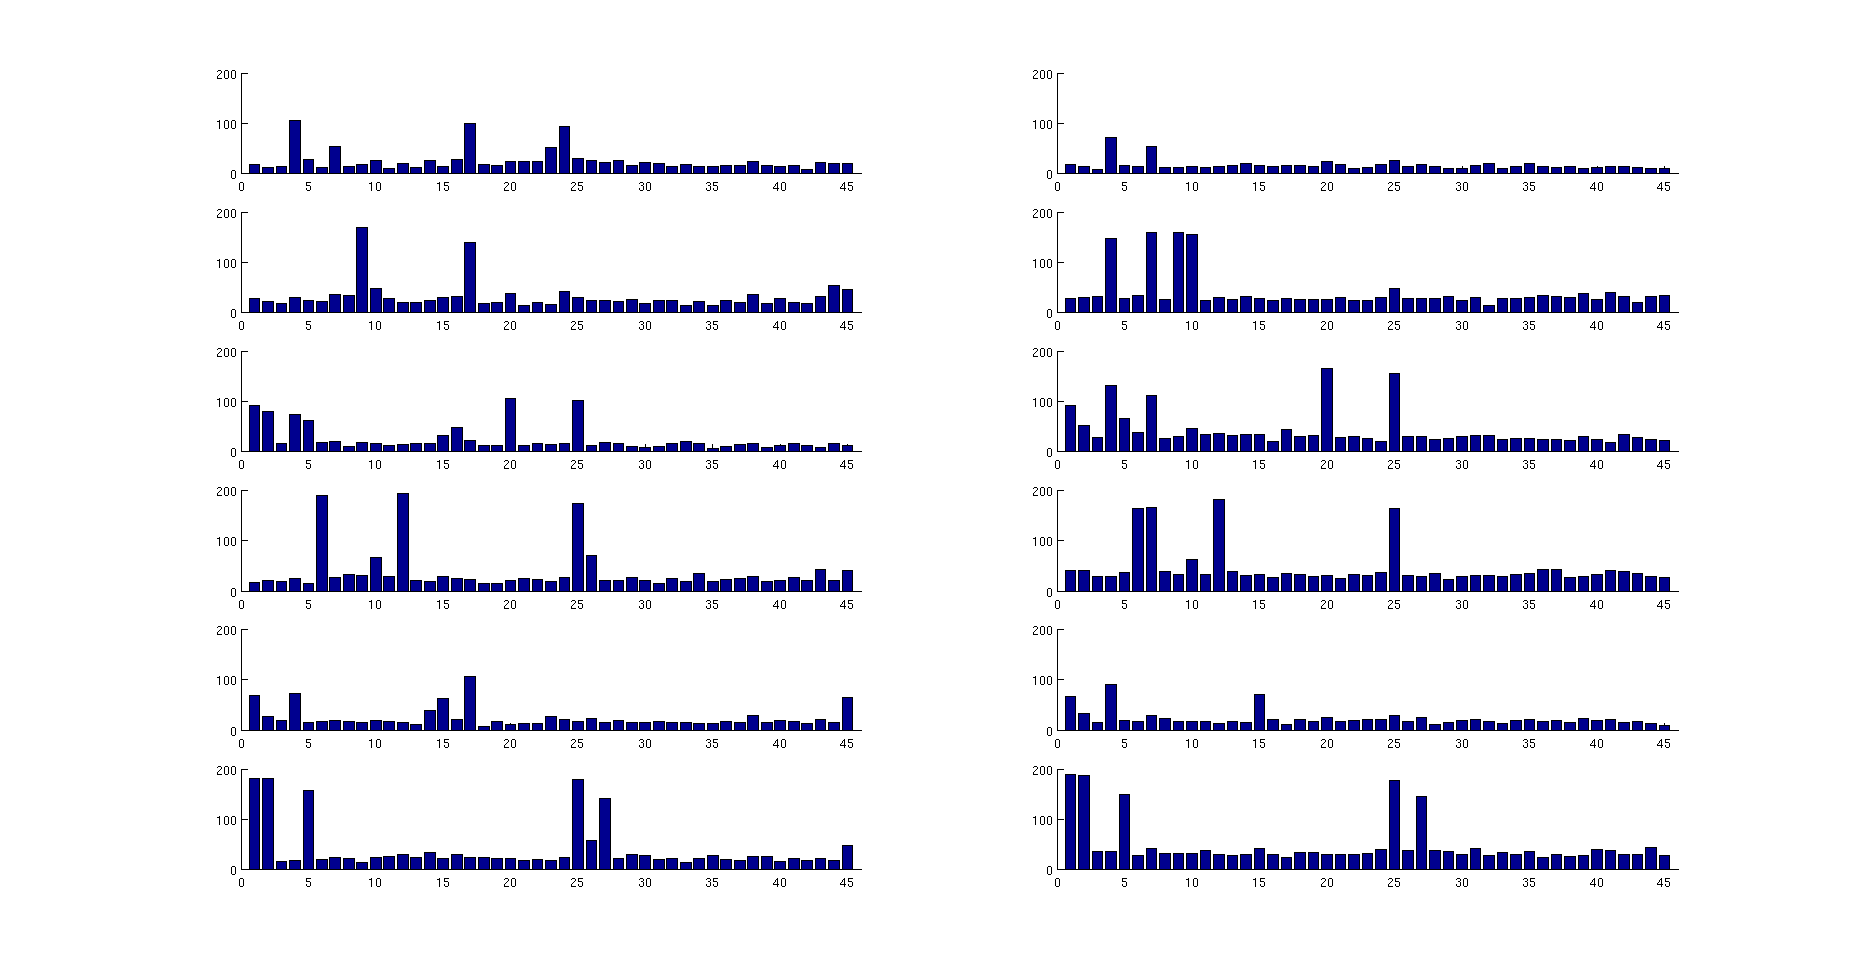
\includegraphics[scale=0.5, angle=90]{images/au_count.png}
	\caption{AU number vs. frequency for emotions 1 to 6 (top to bottom) \\for clean and dirty data (Left and Right)}
	\label{fig:au_counts}
\end{figure}

\section{Performance Results}

Table~\ref{tab:avgClassificationRate} shows the average classification rate of the K-nearest neighbour CBR system on both the clean and the noisy data. We can observe that the CBR system does relatively well on the clean data. This trend can be observed with all similarity measures, with most of the measures reaching classification rates above $80\%$. Note that some of the measures (RR-dissimilarity, Rubbish, Yule dissimilarity) perform badly compared to the others with scores of not exceeding $70\%$. On the other hand, we can observe that other measures such as \emph{shared AUs} or \emph{Weighted Euclidean Distance} perform very well with scores of $86\%$ and $86.7\%$ respectively. The overall performance is thus slightly higher than that found in the Neural Network implementation.

Looking at the performance of the classifier on the noisy data, we can see that the relative order of the distance measures' performances has remained largely the same. However, it is noticeable that all systems' performances have dropped significantly when operating on the new data. The best performance out of all systems is given by the system using the \emph{Shared AUs} distance measure with only $70.3\%$ classification rate. This drop of $15.7$ percentage points is significant and suggests that CBR systems do not operate well on noisy data.
One possible explanation for this is that after being trained initially on the dataset and being provided with the actual labels of the examples, the CBR system continues to learn after the training phase. However, in the test phase the system is not provided with any actual user feedback, which means that the system simply retains its prediction and uses it to make future predictions. This practice is dangerous when the CBR system operates on noisy data. This is because some of the examples in the noisy dataset contain wrong values for AUs which influences how the CBR system computes the similarity of this example. The more misleading examples there are in the CBR system, the less accurate the system becomes. In our test we were unable to validate this as the cause for the significant drop. In fact, the system performs equally well when not retaining examples in the test set. This can be explained by our choice of a relatively small K ($K=3$) for the KNN algorithm and the relatively large number of cases used for training. With only 100 test examples, it is relatively unlikely that the noisy examples will be close enough (by some distance measure) to the other data such that it can significantly influence the classification.

\begin{table}[!ht]
\centering
\begin{tabular}{|l|l|c|c|}
	\cline{3-4}
	\multicolumn{2}{c}{}& \multicolumn{2}{ |c| }{Average Classification Rate}\\
	\cline{3-4}
	\multicolumn{2}{c|}{} & Clean & Noisy \\ \cline{1-4}
    \multirow{11}{*}{Similarity Measure}& Dice Dissimilarity & 0.809 & 0.618   \\ \cline{2-4}
	& Jaccard & 0.809 & 0.618  \\ \cline{2-4}
	& Matching Dissimilarity & 0.86 & 0.703   \\ \cline{2-4}
	& RR Dissimilarity & 0.726  & 0.593  \\ \cline{2-4}
	& RT Dissimilarity & 0.86  & 0.703   \\ \cline{2-4}
	& Rubbish & 0.193 & 0.187  \\ \cline{2-4}
	& Shared AUs & 0.86 & 0.703   \\ \cline{2-4}
	& SS Dissimilarity & 0.809 & 0.618  \\ \cline{2-4}
	& Weighted & 0.863 & 0.709   \\ \cline{2-4}
	& Yule Dissimilarity & 0.796 & 0.595\\ \cline{2-4}
	& Euclidean Distance & 0.86 & 0.703\\ \hline
\end{tabular}
\caption{Average Classification Rate}
\label{tab:avgClassificationRate}
\end{table}

One possible reason for the performance drop in the noisy data is that the noisy data contains attributes that are not relevant to solving the problem (e.g. examples that have the same set of 'core' attributes that can be used to classify it but also have different sets of other attributes that). This means these examples will be spread out when they should actually be close together, and so when a new example needs classifying the examples it should use might be far away from it. The top performing measure, \emph{Shared AUs}, does not take into account what AUs are important for classification so it may indicate that two examples are similar if they share the same irrelevant AUs.

\begin{table}[!ht]
\centering
\begin{tabular}{|l|c|c|c|c|c|c|c|}
	\cline{3-8}
	\multicolumn{2}{c}{}& \multicolumn{6}{ |c| }{Class}\\
	\cline{3-8}
	\multicolumn{2}{c|}{} & 1 Anger & 2 Disgust & 3 Fear & 4 Happiness & 5 Sadness & 6 Surprise\\ \cline{1-8}
	\multirow{2}{*}{Algorithm}& Shared AUs (Clean) & 83.9695 & 81.3131 & 80.5085 & 94.8837 & 76.5152 & 91.7476 \\ \cline{2-8}  
	& Shared AUs (Noisy) & 45.4545 & 79.1444 & 64.1711 & 78.3654 & 51.8182 & 79.5455 \\ \cline{2-8} 
		& Weighted (Clean) & 79.3893 & 85.3535 & 82.2034 & 94.8837 & 78.0303 & 90.2913\\ \cline{2-8} 
	& Weighted (Noisy) & 39.7727 & 82.3529 & 65.7754 & 78.3654 & 55.4545 & 78.6364\\ \cline{2-8}
			& Dice (Clean) & 79.3893 & 76.7677 & 73.7288 & 91.6279 & 65.1515 & 88.8350\\ \cline{2-8} 
	& Dice (Noisy) & 28.4091 & 80.2139 & 54.5455 & 69.2308 & 26.36363 & 76.3636\\ \cline{2-8}
			& Yule (Clean) & 52.6718 & 86.8687 & 72.0339 & 87.9070 & 78.7879 & 85.9223\\ \cline{2-8}
	& Yule (Noisy) & 72.7273 & 53.4759 & 37.4332 & 75.0000 & 38.1818 & 74.0909\\ \hline

\end{tabular}
\caption{Precision Per Class}
\label{tab:precisionPerClass}
\end{table}

\begin{table}[!ht]
\centering
\begin{tabular}{|l|c|c|c|c|c|c|c|}
	\cline{3-8}
	\multicolumn{2}{c}{}& \multicolumn{6}{ |c| }{Class}\\
	\cline{3-8}
	\multicolumn{2}{c|}{} & 1 Anger & 2 Disgust & 3 Fear & 4 Happiness & 5 Sadness & 6 Surprise\\ \cline{1-8}
	\multirow{2}{*}{Algorithm}& Shared AUs (Clean) & 78.0142  & 79.3103 & 85.5856 & 92.3077 & 84.1667  & 92.6471 \\ \cline{2-8}  
	& Shared AUs (Noisy) & 33.3333 & 72.9064 & 63.4921 & 84.8958 & 65.5172 & 83.7321 \\ \cline{2-8} 
		& Weighted (Clean) & 80.6202 & 80.0948 & 83.6207 & 92.3077 & 83.0645 & 93.4673 \\ \cline{2-8} 
	& Weighted (Noisy) & 33.9806 & 76.6169 & 63.7306 & 84.0206 & 64.2105 & 80.8411 \\ \cline{2-8}
			& Dice (Clean) & 66.2420 & 76.7677 & 73.1092 & 90.3670 & 84.3137 & 88.8350\\ \cline{2-8} 
	& Dice (Noisy) & 25.5102 & 62.7615 & 52.3077 & 77.4194 & 59.1837 & 72.1030 \\ \cline{2-8}
			& Yule (Clean) & 81.1765  & 73.5043 & 75.8929 & 95.4545 & 57.1429 & 93.6508\\ \cline{2-8}
	& Yule (Noisy) & 20.8469 & 81.3008 & 66.0377 & 86.1878 & 47.7273 & 83.5897\\ \hline

\end{tabular}
\caption{Recall Per Class}
\label{tab:recallPerClass}
\end{table}

\begin{table}[!ht]
\centering
\begin{tabular}{|l|c|c|c|c|c|c|c|}
	\cline{3-8}
	\multicolumn{2}{c}{}& \multicolumn{6}{ |c| }{Class}\\
	\cline{3-8}
	\multicolumn{2}{c|}{} & 1 Anger & 2 Disgust & 3 Fear & 4 Happiness & 5 Sadness & 6 Surprise\\ \cline{1-8}
	\multirow{2}{*}{Algorithm}& Shared AUs (Clean) & 80.8824  & 80.2993 & 82.9694 & 93.5701 & 80.1587 & 92.1951 \\ \cline{2-8}  
	& Shared AUs (Noisy) & 38.4615 & 75.8974 & 63.8298 & 81.5000 & 57.8680 & 81.5851\\ \cline{2-8} 
		& Weighted (Clean) & 80.0000 & 82.6406 & 82.9060 & 93.5780 & 80.4688 & 91.8519\\ \cline{2-8} 
	& Weighted (Noisy) & 36.6492 & 79.3814 & 64.7368 & 81.0945 & 59.5122 & 79.7235\\ \cline{2-8}
			& Dice (Clean) & 72.2222 & 76.7677 & 73.4177 & 90.9931 & 73.5043 & 88.8350 \\ \cline{2-8} 
	& Dice (Noisy) & 45.4545 & 83.7093 & 67.5393 & 85.9223 & 56.5217 & 85.0112\\ \cline{2-8}
			& Yule (Clean) & 63.8889 & 79.6296 & 739130 & 91.5254 & 66.2420 & 89.6203 \\ \cline{2-8}
	& Yule (Noisy) & 32.4051 & 64.5161 & 47.7816 & 80.2057 & 42.4242 & 78.5542\\ \hline


\end{tabular}
\caption{F1 Measure Per Class}
\label{tab:f1PerClass}
\end{table}

Tables \ref{tab:precisionPerClass}, \ref{tab:recallPerClass}, and \ref{tab:f1PerClass} show the precision rates, recall rates and $F_1$ measures per class. The tables confirm again that it appears to be relatively easy to learn to identify \emph{happiness} and \emph{surprise}. Even though there is a noticeable drop in performance for all emotions, emotions such as \emph{happiness} and \emph{surprise} can still be classified relatively easily.

It is also noticeable that the CBR managed to identify more difficult emotions such as \emph{anger}, \emph{disgust} or\emph{fear} in the clean data with relatively high recall, precision and $F_1$ scores. However, the drop in performance for the clean data is especially prevalent for these attributes.

Tables \ref{tab:sharedAUsCleanConfusion}, \ref{tab:sharedAUsNoisyConfusion}, \ref{tab:weightedCleanConfusion}, \ref{tab:weightedNoisyConfusion}, \ref{tab:diceCleanConfusion}, \ref{tab:diceNoisyConfusion}, \ref{tab:yuleCleanConfusion}, \ref{tab:yuleNoisyConfusion} show the confusion matrices for the \emph{shared AUs}, \emph{weighted}, \emph{Dice Dissimilarity} and \emph{Yule Dissimilarity} distance measures.

\begin{table}[!ht]
\centering
\begin{tabular}{|l|l|c|c|c|c|c|c|}
	\cline{3-8}
	\multicolumn{2}{c}{}& \multicolumn{6}{ |c| }{Predicted class}\\
	\cline{3-8}
	\multicolumn{2}{c|}{} & 1 Anger & 2 Disgust & 3 Fear & 4 Happiness & 5 Sadness & 6 Surprise\\ \cline{1-8}
	\multirow{6}{*}{Actual class}& 1 Anger & 110 & 8 & 4 & 2 & 6 & 1 \\ \cline{2-8}
	& 2 Disgust & 14 & 161 & 1 & 8 & 13 & 1\\ \cline{2-8}
	& 3 Fear & 7 & 6 & 95 & 0 & 0 & 10 \\ \cline{2-8}
	& 4 Happiness & 0 & 9 & 0 & 204 & 0 & 2 \\ \cline{2-8}
	& 5 Sadness & 8 & 16 & 2 & 4 & 101 & 1 \\ \cline{2-8}
	& 6 Surprise & 1 & 3 & 9 & 3 & 0 & 189\\ \hline
\end{tabular}
\caption{Confusion Matrix - Shared AUs - Clean Data}
\label{tab:sharedAUsCleanConfusion}
\end{table}

\begin{table}[!ht]
\centering
\begin{tabular}{|l|l|c|c|c|c|c|c|}
	\cline{3-8}
	\multicolumn{2}{c}{}& \multicolumn{6}{ |c| }{Predicted class}\\
	\cline{3-8}
	\multicolumn{2}{c|}{} & 1 Anger & 2 Disgust & 3 Fear & 4 Happiness & 5 Sadness & 6 Surprise\\ \cline{1-8}
	\multirow{6}{*}{Actual class}& 1 Anger & 40 & 13 & 17 & 4 & 10 & 4 \\ \cline{2-8}
	& 2 Disgust & 15 & 148 & 16 & 3 & 4 & 1\\ \cline{2-8}
	& 3 Fear & 17 & 16 & 120 & 11 & 7 & 16\\ \cline{2-8}
	& 4 Happiness & 13 & 10 & 13 & 163 & 1 & 8 \\ \cline{2-8}
	& 5 Sadness & 26 & 12 & 7 & 3 & 57 & 5 \\ \cline{2-8}
	& 6 Surprise & 9 & 4 & 16 & 8 & 8 & 175\\ \hline
\end{tabular}
\caption{Confusion Matrix - Shared AUs - Noisy Data}
\label{tab:sharedAUsNoisyConfusion}
\end{table}

\begin{table}[!ht]
\centering
\begin{tabular}{|l|l|c|c|c|c|c|c|}
	\cline{3-8}
	\multicolumn{2}{c}{}& \multicolumn{6}{ |c| }{Predicted class}\\
	\cline{3-8}
	\multicolumn{2}{c|}{} & 1 Anger & 2 Disgust & 3 Fear & 4 Happiness & 5 Sadness & 6 Surprise\\ \cline{1-8}
	\multirow{6}{*}{Actual class}& 1 Anger & 104 & 12 & 4 & 2 & 8 & 1 \\ \cline{2-8}
	& 2 Disgust & 10 & 169 & 1 & 4 & 13 & 1\\ \cline{2-8}
	& 3 Fear & 6 & 5 & 97 & 1 & 0 & 9 \\ \cline{2-8}
	& 4 Happiness & 2 & 7 & 1 & 204 & 0 & 1 \\ \cline{2-8}
	& 5 Sadness & 5 & 16 & 3 & 4 & 103 & 1 \\ \cline{2-8}
	& 6 Surprise & 2 & 2 & 10 & 6 & 0 & 186\\ \hline
\end{tabular}
\caption{Confusion Matrix - Weighted - Clean Data}
\label{tab:weightedCleanConfusion}
\end{table}

\begin{table}[!ht]
\centering
\begin{tabular}{|l|l|c|c|c|c|c|c|}
	\cline{3-8}
	\multicolumn{2}{c}{}& \multicolumn{6}{ |c| }{Predicted class}\\
	\cline{3-8}
	\multicolumn{2}{c|}{} & 1 Anger & 2 Disgust & 3 Fear & 4 Happiness & 5 Sadness & 6 Surprise\\ \cline{1-8}
	\multirow{6}{*}{Actual class}& 1 Anger & 35 & 11 & 22 & 3 & 13 & 4 \\ \cline{2-8}
	& 2 Disgust & 1 & 154 & 12 & 6 & 3 & 1\\ \cline{2-8}
	& 3 Fear & 16 & 12 & 123 & 9 & 7 & 20 \\ \cline{2-8}
	& 4 Happiness & 10 & 12 & 12 & 163 & 2 & 9 \\ \cline{2-8}
	& 5 Sadness & 26 & 5 & 8 & 3 & 61 & 7 \\ \cline{2-8}
	& 6 Surprise & 5 & 7 & 16 & 10 & 9 & 173\\ \hline
\end{tabular}
\caption{Confusion Matrix - Weighted - Noisy Data}
\label{tab:weightedNoisyConfusion}
\end{table}

\begin{table}[!ht]
\centering
\begin{tabular}{|l|l|c|c|c|c|c|c|}
	\cline{3-8}
	\multicolumn{2}{c}{}& \multicolumn{6}{ |c| }{Predicted class}\\
	\cline{3-8}
	\multicolumn{2}{c|}{} & 1 Anger & 2 Disgust & 3 Fear & 4 Happiness & 5 Sadness & 6 Surprise\\ \cline{1-8}
	\multirow{6}{*}{Actual class}& 1 Anger & 104 & 12 & 5 & 2 & 6 & 2 \\ \cline{2-8}
	& 2 Disgust & 23 & 152 & 3 & 9 & 10 & 1\\ \cline{2-8}
	& 3 Fear & 11 & 4 & 87 & 1 & 0 & 15 \\ \cline{2-8}
	& 4 Happiness & 5 & 6 & 4 & 197 & 0 & 3 \\ \cline{2-8}
	& 5 Sadness & 11 & 21 & 8 & 4 & 86 & 2 \\ \cline{2-8}
	& 6 Surprise & 3 & 3 & 12 & 5 & 0 & 183\\ \hline
\end{tabular}
\caption{Confusion Matrix - Dice Dissimilarity - Clean Data}
\label{tab:diceCleanConfusion}
\end{table}

\begin{table}[!ht]
\centering
\begin{tabular}{|l|l|c|c|c|c|c|c|}
	\cline{3-8}
	\multicolumn{2}{c}{}& \multicolumn{6}{ |c| }{Predicted class}\\
	\cline{3-8}
	\multicolumn{2}{c|}{} & 1 Anger & 2 Disgust & 3 Fear & 4 Happiness & 5 Sadness & 6 Surprise\\ \cline{1-8}
	\multirow{6}{*}{Actual class}& 1 Anger & 25 & 21 & 26 & 5 & 6 & 5 \\ \cline{2-8}
	& 2 Disgust & 17 & 150 & 8 & 6 & 3 & 3\\ \cline{2-8}
	& 3 Fear & 23 & 22 & 102 & 14 & 3 & 23 \\ \cline{2-8}
	& 4 Happiness & 8 & 20 & 20 & 144 & 2 & 14 \\ \cline{2-8}
	& 5 Sadness & 19 & 15 & 20 & 7 & 29 & 20 \\ \cline{2-8}
	& 6 Surprise & 6 & 11 & 19 & 10 & 6 & 168\\ \hline
\end{tabular}
\caption{Confusion Matrix -  Dice Dissimilarity - Noisy Data}
\label{tab:diceNoisyConfusion}
\end{table}

\begin{table}[!ht]
\centering
\begin{tabular}{|l|l|c|c|c|c|c|c|}
	\cline{3-8}
	\multicolumn{2}{c}{}& \multicolumn{6}{ |c| }{Predicted class}\\
	\cline{3-8}
	\multicolumn{2}{c|}{} & 1 Anger & 2 Disgust & 3 Fear & 4 Happiness & 5 Sadness & 6 Surprise\\ \cline{1-8}
	\multirow{6}{*}{Actual class}& 1 Anger & 69 & 16 & 6 & 1 & 38 & 1 \\ \cline{2-8}
	& 2 Disgust & 8 & 172 & 4 & 2 & 12 & 0\\ \cline{2-8}
	& 3 Fear & 4 & 7 & 85 & 1 & 13 & 8 \\ \cline{2-8}
	& 4 Happiness & 2 & 13 & 2 & 189 & 7 & 2 \\ \cline{2-8}
	& 5 Sadness & 1 & 22 & 3 & 1 & 104 & 1 \\ \cline{2-8}
	& 6 Surprise & 1 & 4 & 12 & 4 & 8 & 177\\ \hline
\end{tabular}
\caption{Confusion Matrix - Yule Dissimilarity - Clean Data}
\label{tab:yuleCleanConfusion}
\end{table}

\begin{table}[!ht]
\centering
\begin{tabular}{|l|l|c|c|c|c|c|c|}
	\cline{3-8}
	\multicolumn{2}{c}{}& \multicolumn{6}{ |c| }{Predicted class}\\
	\cline{3-8}
	\multicolumn{2}{c|}{} & 1 Anger & 2 Disgust & 3 Fear & 4 Happiness & 5 Sadness & 6 Surprise\\ \cline{1-8}
	\multirow{6}{*}{Actual class}& 1 Anger & 64 & 6 & 4 & 2 & 11 & 1 \\ \cline{2-8}
	& 2 Disgust & 72 & 100 & 6 & 3 & 4 & 2\\ \cline{2-8}
	& 3 Fear & 76 & 6 & 70 & 7 & 11 & 17 \\ \cline{2-8}
	& 4 Happiness & 27 & 8 & 9 & 156 & 3 & 5 \\ \cline{2-8}
	& 5 Sadness & 50 & 2 & 7 & 2 & 42 & 7 \\ \cline{2-8}
	& 6 Surprise & 18 & 1 & 10 & 11 & 17 & 163\\ \hline
\end{tabular}
\caption{Confusion Matrix - Yule Dissimilarity - Noisy Data}
\label{tab:yuleNoisyConfusion}
\end{table}

\begin{figure}[!ht]
	\centering
	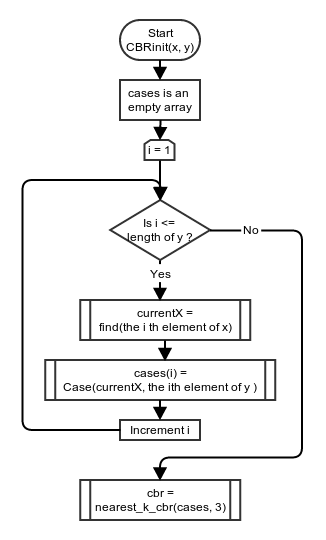
\includegraphics[scale=0.7]{images/flow_chart/cbrinit.png}
	\caption{Flowchart of \tt{CBRinit}}
	\label{fig:cbrinit}
\end{figure}

\begin{figure}[!ht]
	\centering
	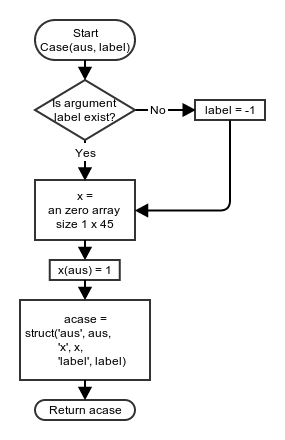
\includegraphics[scale=0.7]{images/flow_chart/case.png}
	\caption{Flowchart of \tt{Case}}
	\label{fig:Case}
\end{figure}

\begin{figure}[!ht]
	\centering
	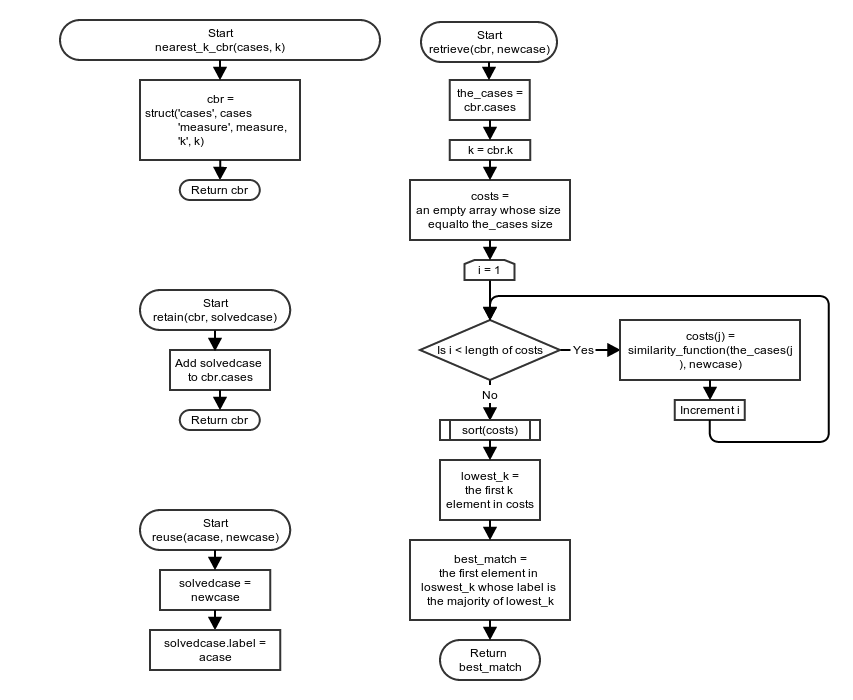
\includegraphics[scale=0.6]{images/flow_chart/nearest_k_cbr.png}
	\caption{Flowchart of \tt{nearest\_k\_cbr}}
	\label{fig:nearest_k_cbr}
\end{figure}

\begin{figure}[!ht]
	\centering
	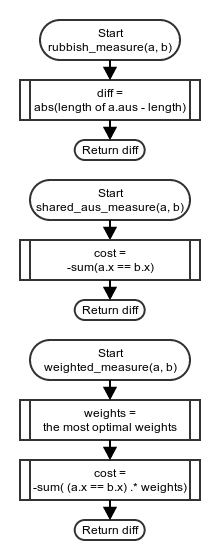
\includegraphics[scale=0.7]{images/flow_chart/measure_function.png}
	\caption{Flowchart of \tt{similarity\_function}}
	\label{fig:measure_function}
\end{figure}

\begin{figure}[!ht]
	\centering
	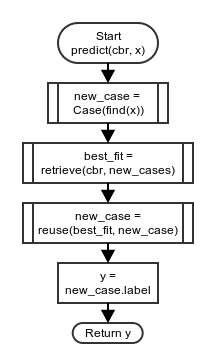
\includegraphics[scale=0.7]{images/flow_chart/predict.png}
	\caption{Flowchart of \tt{predict}}
	\label{fig:predict}
\end{figure}

\begin{figure}[!ht]
	\centering
	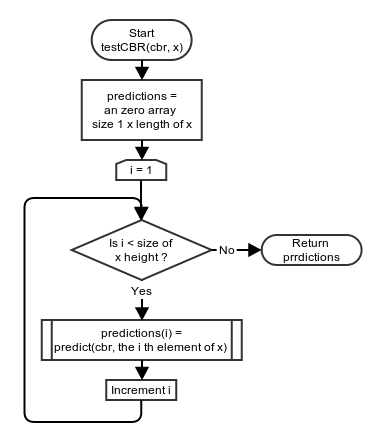
\includegraphics[scale=0.7]{images/flow_chart/testcbr.png}
	\caption{Flowchart of \tt{testCBR}}
	\label{fig:testcbr}
\end{figure}


\bibliography{case_based_reasoning}
\bibliographystyle{plain}

\end{document}
